\chapter{Modelos epidemiológicos} \label{chp:epi_models}

\section{Modelos compartimentales}

Para modelar la propagación de enfermedades infecciosas, es muy habitual utilizar modelos compartimentales basados en ecuaciones diferenciales. Estos pueden ser utilizados para predecir y comprender situaciones epidemiológicas, ayudar a la toma de decisiones y simular situaciones hipotéticas así como también se pueden utilizar para estimar parámetros. Su origen se remonta a los años 20 del siglo pasado y suele atribuirse a \cite{Kermack1927}. Estos consisten en modelar la población distinguiendo subpoblaciones de acuerdo a categorías epidemiológicas. Por ejemplo, el emblemático modelo SIR, distingue a las subpoblaciones susceptible ($S$), infectada ($I$) y recuperada ($R$). Este se puede expresar mediante el siguiente sistema de ecuaciones diferenciales,
\begin{align} \label{eq:sir}
    \frac{\partial S}{\partial t} &= -\beta \frac{SI}{N}\\
    \frac{\partial I}{\partial t} &= \beta \frac{SI}{N} - \gamma I \\
    \frac{\partial R}{\partial t} &= \gamma I
\end{align}
Estas ecuaciones suponen una población constante de tamaño $N$: notemos que las ecuaciones suman 0 por lo que la población total se mantiene. La velocidad con que los individuos susceptibles se infectan es proporcional a la cantidad total de susceptibles, $S$ y a la proporción de infectados de la población $\frac{I}{N}$. La constante de proporcionalidad $\beta$ es llamada la tasa de infección y cuantifica la transmisibilidad de la enfermedad. Por su parte, la velocidad con que los infectados se recuperan es proporcional a la cantidad de infectados y la constante de proporcionalidad $\gamma$ es llamada tasa de recuperación. El sistema resulta en una epidemia cuando $\frac{\partial I}{\partial t} > 0$ y esto sucede cuando $\frac{\beta S(0)}{\gamma} > N$. El número reproductivo básico, $R_0$ en un modelo epidemiológico suele definirse como la cantidad de infectados directos que provocaría un infectado en una población totalmente susceptible. En este caso se puede computar de manera explícita como $R_0 = \frac{\beta}{\gamma}$. El umbral en el comportamiento del sistema depende entonces de este valor pues para que se de un pico epidémico se debe dar que $R_0 S(0) > N$.  En general $t = 0$ representa un momento en el que la enfermedad está surgiendo y por lo tanto $S(0) \approx N$. Debido a esto se suele considerar que la condición para tener una epidemia es cuando $R_0 > 1$. 

El modelo SIR, aunque sencillo, merece mención pues tiene los elementos básicos con los que se puede construir un modelo compartimental. Como vimos, la entrada y salida de cada compartimento se describe con una ecuación diferencial y con esta idea se pueden diseñar distintas estructuras de subpoblaciones para describir las situaciones que se deseen modelar. Es común ver en este tipo de modelos la subpoblación de los decesos $D$ que permite distinguir a la porción de la población que muere a causa de la enfermedad, o la subpoblación de los expuestos $E$ se suele ver en modelos para enfermedades virales en que las personas se infectan e incuban el virus sin ser infecciosas antes de pasar al compartimento $I$. De esta manera tenemos modelos como el SEIRD que considera estas subpoblaciones, o el SIS que no tiene en cuenta una categoría de recuperados sino que considera que los individuos, al curarse de la enfermedad vuelven a ser susceptibles. Otros consideran compartimentos que corresponden a los inmunizados mediante vacunación. Habitualmente se representa con un diagrama de flujo cuales son los compartimientos y qué direcciones toma el cambio de estado epidemiológico de acuerdo a las características de la enfermedad. Por ejemplo, en la Figura \ref{dia:sir} podemos ver esta representación para un modelo SIR.
\begin{figure}[h]
    \centering
    \begin{tikzpicture}[node distance=3.5cm, auto]
        \tikzstyle{block} = [rectangle, draw, fill=blue!20, 
        text width=4em, text centered, rounded corners, minimum height=3em]
        \tikzset{line/.style={draw, very thick, color=black!100, -latex'}}
        
        \node [block] (S){$S$};
        \node [block, right of=S] (I){$I$};
        \node [block, right of=I] (R){$R$};
        
        \path [line] (S) -- node {\scriptsize $\beta \frac{SI}{N}$} (I);
        \path [line] (I) -- node {\scriptsize $\gamma I$} (R);

    \end{tikzpicture}
    \caption{Diagrama para un modelo SIR} \label{dia:sir}
\end{figure}

En, general podemos distinguir 3 tipos distintos de compartimentos: aquellos que actúan de fuente, es decir que solo decrecen o se mantienen, y por lo tanto los términos en las ecuaciones diferenciales son sólo negativos, los compartimentos intermedios, cuyas ecuaciones incluyen términos positivos y negativos y finalmente los compartimentos que actúan de sumidero, es decir que sólo crecen o se mantienen los cuales sólo incluyen términos positivos. Por ejemplo, en el modelo SIR el compartimento $S$ actúa a modo de fuente, $I$ es un compartimento intermedio y $R$ actúa de sumidero. Típicamente las trayectorias de las fuentes tienen una forma sigmoidea decreciente y las de los sumideros son sigmoideas decrecientes mientras que los compartimientos intermedios suelen exhibir un comportamiento con forma de campana. En la figura \ref{fig:sir_example} se puede observar esto en las trayectorias generadas por un modelo SIR.

\begin{figure}[h]
    \centering
    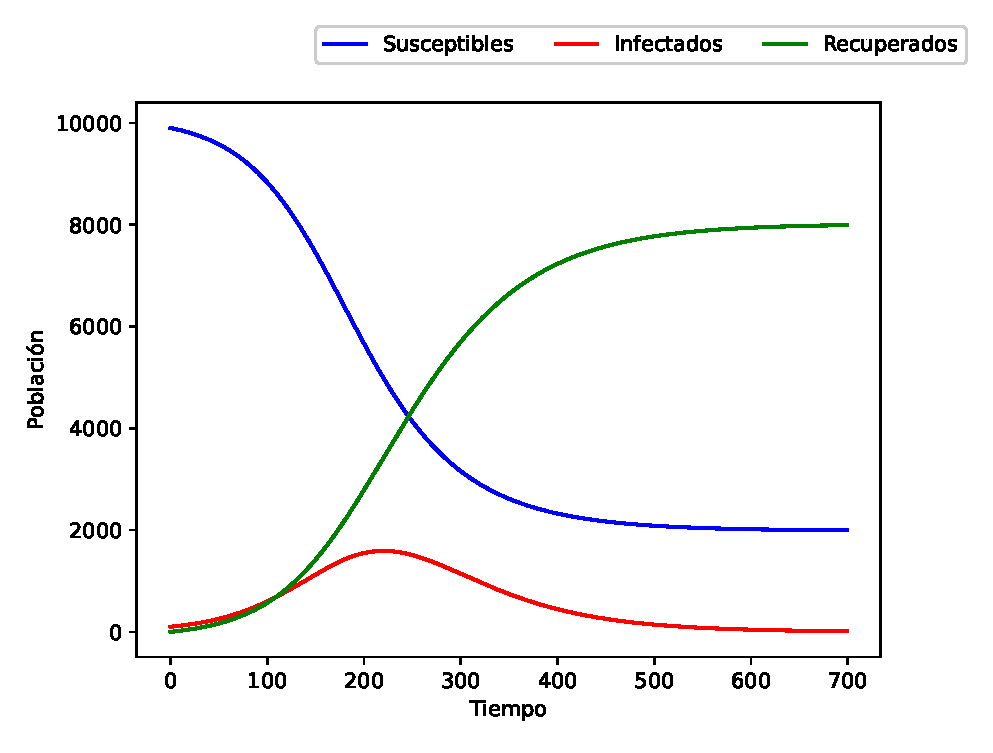
\includegraphics[width=0.75\textwidth]{sir_example.eps}
    \caption{Trayectorias de susceptibles, infectados y recuperados para un modelo SIR básico}
    \label{fig:sir_example}
\end{figure}

La incorporación de compartimentos le da gran adaptabilidad a estos modelos. Sin embargo, se considera que las subpoblaciones representadas en cada uno de estos compartimentos se mezcla de manera homogénea con lo cual no se representan los efectos que provienen de las complejidades del comportamiento de los individuos. Como veremos más adelante, los modelos basados en agentes se focalizan en modelar cada individuo de manera de dar cuenta de las consecuencias de las interacciones en esta micro-escala. Por otro lado, la representación mediante ecuaciones da la posibilidad de analizar formalmente el comportamiento del sistema para, por ejemplo, identificar puntos de equilibrio, umbrales entre distintos tipos de soluciones o cálculos explícitos del número reproductivo básico \citep{Murray2007}.

Además de la incorporación de subpoblaciones relacionadas a los estados epidemiológicos, los modelos compartimentales pueden incluir otras características. Por ejemplo, se pueden utilizar variables espaciales acopladas a términos de difusión en las ecuaciones para representar la dispersión territorial de las enfermedades \citep{Noble1974}. También se utiliza estratificación por edades para diferenciar el efecto de la enfermedad en distintos sectores de la población y codificar el contacto entre los distintos rangos etarios \citep{Hethcote2000}. Además se puede modelar la espacialidad a través de la determinación de áreas, por ejemplo barrios en una ciudad, cada una con sus propias subpoblaciones de susceptibles, infectados etc. y describiendo la interacción entre estos lugares \citep{Klepac2018}. Con el advenimiento de la pandemia de COVID-19 se desarrollaron un gran número de modelos compartimentales con características especiales para expresar determinados rasgos propios de esta enfermedad y que se han utilizado para diversos fines tales como la estimación de parámetros epidemiológicos, la evaluación de medidas de control o la predicción de tendencias en los picos de contagios. Por ejemplo, el modelo de \cite{Evensen2020} utiliza estratificación por edades y compartimentos para representar de subpoblaciones bajo distintos tipos de cuarentena y es utilizado para estimar $R_0$ y hacer predicciones en distintos escenarios en diferentes países. El modelo de \cite{Arenas2020} también incluye estratificación por edades pero también incorpora patrones de movimiento en distintas regiones de España, compartimentos para los hospitalizados y otras características incluidas para adaptar el esquema al COVID-19. En general, cuando tenemos una segmentación de la población en $K$ grupos (ya sea rango etario, locación o alguna otro) tenemos una réplica del sistema de ecuaciones por cada uno de ellos. La interacción entre estos se representa mediante una matriz $K \times K$. Si extendemos las ecuaciones del modelo SIR a un modelo multi-grupos tendremos las siguientes ecuaciones para $i=1, ..., K$:
\begin{align}
    \frac{\partial S_i}{\partial t} &= -\beta \sum_{j=1}^{K}c_{ij}\frac{S_i I_j}{N}\\
    \frac{\partial I_i}{\partial t} &= \beta \sum_{j=1}^{K}c_{ij}\frac{S_i I_j}{N} - \gamma I_i \\
    \frac{\partial R_i}{\partial t} &= \gamma I_i
\end{align}
donde $c$ es la matriz de conectividad, de manera que la interacción entre el grupo $i$ y y el $j$ está cuantificado por $c_{ij}$.

\section{Inferencia en modelos compartimentales}

Los modelos epidemiológicos por sí solos pueden ser útiles para entender algunos fenómenos respecto a las dinámicas de contagio o los posibles efectos de medidas de control en escenarios hipotéticos. Sin embargo, la parametrización que se utilice puede cambiar drásticamente el comportamiento de los modelos y se hace importante la estimación de parámetros para un mejor ajuste del modelo a los datos o para obtener pronósticos más certeros. Por estos motivos es normal acoplar al modelo alguna técnica de inferencia que permita realizar esta tarea. En particular, la asimilación de datos provee, por un lado técnicas para estimar parámetros como el estado aumentado y por otro mejora los pronósticos de las mismas variables de estado incorporando la información de las observaciones. Además de esto, la asimilación de datos está diseñada de manera que es natural el tratamiento de variables no observadas, y en un sistema epidemiológico es normal que haya observaciones incompletas (por ejemplo que sólo se observe la subpoblación de infectados y muertos pero no se observe ninguna de las otras). 

Los trabajos \cite{Ionides2006} y posteriormente \cite{Shaman2012, Shaman2013} constituyen excelentes ejemplos de la aplicación de técnicas modernas de asimilación de datos en modelos epidemiológicos. En \cite{Ionides2006} se utiliza, para un modelo compartimental para el cólera, la técnica de filtros iterados para estimar variables de estado y parámetros estocásticos y físicos. La técnica está basada en el uso de estado aumentado pero con la variante de que se pasa repetidas veces el filtro y en cada iteración se reduce la varianza del parámetro de estado aumentado de tal manera que el valor se va estabilizando en un valor fijo que corresponde al máximo de la verosimilitud. Además se utiliza un filtro de partículas lo cual permite la inferencia en escenarios de no linealidad. Por otro lado, en los trabajos de \cite{Shaman2012, Shaman2013} se aplica el EAKF, una variante del EnKF, a un modelo SIRS para predecir picos de gripe y estimar parámetros relacionados a $R_0$ mediante estado aumentado. Más recientemente, ha habido aplicaciones para modelos de COVID-19. En \cite{Li2020} se utilizan filtros iterados pero con el EAKF para estimar casos no reportados en China. en \cite{Evensen2020} se aplica una técnica basada en suavizadores de Kalman por ensambles llamada ESMDA (\textit{Ensemble Smoother with Multiple Data Assimilation}) para calibrar la parametrización del modelo y, en particular, estimar el número de reproducción efectivo en un modelo compartimental. Por otro lado en \cite{Ghostine2021} se utiliza el EnKF para estudiar el efecto de la vacunación con datos de Arabia Saudita.

A pesar de que las aplicaciones de técnicas de asimilación de datos a modelos epidemiológicos se comienzan a popularizar no se ha hecho particular foco en la estimación de errores observacionales y de modelo. Estas cantidades no sólo tienen interés en sí mismo para la comprensión de las incertezas del sistema sino que, como hemos visto en el Capítulo \ref{chp:error_treatment}, también afectan en la performance del sistema. En particular, el error observacional en modelos epidemiológicos tiene la complejidad de estar relacionado al reporte de casos lo cual puede ser una fuente de información poco precisa y cuya incerteza varía en el tiempo. Por estas cualidades realizamos para esta tesis experimentos preliminares de aplicación de el algoritmo EM online presentado en la sección \ref{sec:onlineEM} cuyos resultados presentamos a continuación.

\subsection{Experimento: observaciones sintéticas} \label{sec:online_em_seird_synthetic}
Para mostrar algunas de las capacidades de el EnKF acoplado con el EM online en un modelo epidemiológico realizamos un experimento con observaciones sintéticas sobre un modelo SEIRD definido por las siguientes ecuaciones diferenciales:
\begin{align} \label{eq:seird}
    \frac{\partial S}{\partial t} &= -\beta \frac{SI}{N}\\
    \frac{\partial E}{\partial t} &= \beta \frac{SI}{N} - \gamma_E E \\
    \frac{\partial I}{\partial t} &= \gamma_E E - \gamma_I I \\
    \frac{\partial R}{\partial t} &= \alpha \gamma_I I \\
    \frac{\partial D}{\partial t} &= (1-\alpha) \gamma_I I
\end{align}
donde $S$, $E$, $I$, $R$ y $D$ representan a los susceptibles, expuestos, infectados, recuperados y muertos respectivamente. $\beta$ es la tasa de infección, $\gamma_E$ determina la velocidad con que los expuestos pasan a ser infectados y $\gamma_I$ la tasa a la que los infectados se recuperan o mueren. La proporción de infectados que mueren es $\alpha$ y la que se recupera $1 - \alpha$. El sistema se puede representar mediante el diagrama de la Figura \ref{dia:seird}. 

\begin{figure}[h]
    \centering
    \begin{tikzpicture}[node distance=3.5cm, auto]
        \tikzstyle{block} = [rectangle, draw, fill=blue!20, 
        text width=4em, text centered, rounded corners, minimum height=3em]
        \tikzset{line/.style={draw, very thick, color=black!100, -latex'}}
        
        \node [block] (S){$S$};
        \node [block, right of=S] (E){$E$};
        \node [block, right of=E] (I){$I$};
        \node [block, above right = 0.1cm and 1cm of I] (R){$R$};
        \node [block, below right = 0.1cm and 1cm of I] (D){$D$};
        
        \path [line] (S) --  node {\scriptsize $\beta \frac{SI}{N}$} (E);
        \path [line] (E) --  node {\scriptsize $\gamma_E E$} (I);
        \path [line] (I) --  node {\scriptsize $\alpha \gamma_I I$} (R);
        \path [line] (I) --  node {\scriptsize $(1-\alpha) \gamma_I I$} (D);

    \end{tikzpicture}
    \caption{Diagrama para un modelo SEIRD} \label{dia:seird}
\end{figure}

Consideramos que las observaciones corresponden a los infectados acumulados y a los muertos. Los infectados acumulados, que llamaremos $I_{tot}$ pueden ser computados como la suma de las variables $I$, $R$ y $D$. Por lo tanto el operador observacional se puede escribir en forma matricial como:
\begin{align*}
    \v H = 
    \begin{pmatrix}
        0 & 0 & 1 & 1 & 1 \\
        0 & 0 & 0 & 0 & 1 
    \end{pmatrix}.
\end{align*}
\begin{figure}[h]
    \centering
    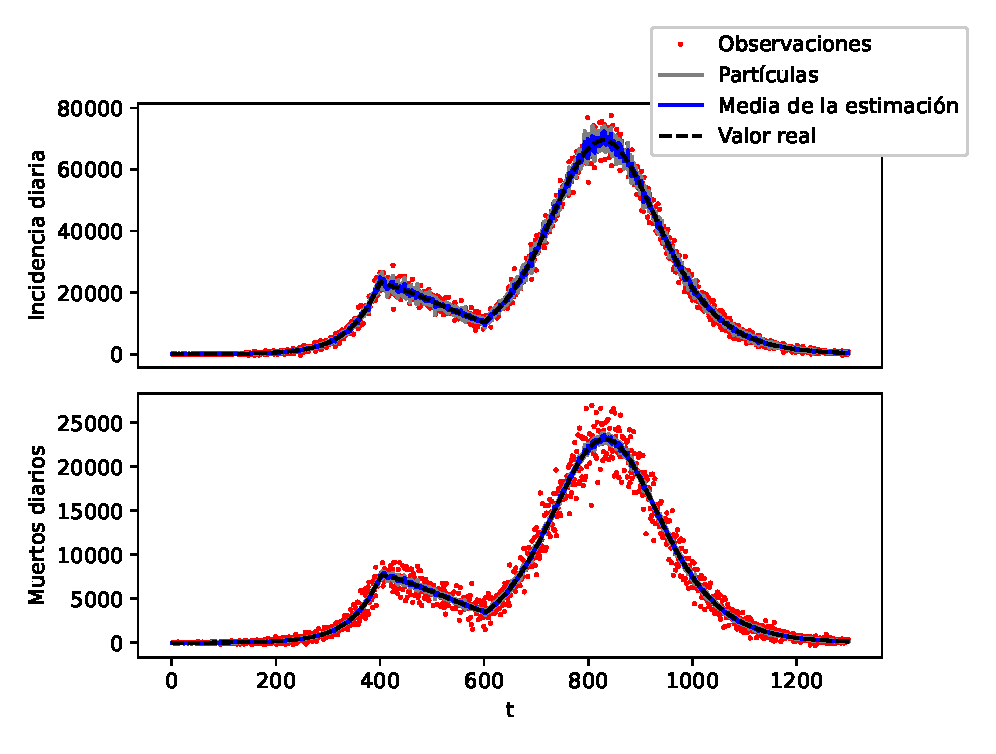
\includegraphics[width=0.75\textwidth]{figs/seird_online_em_aug_state_state_vars.eps}
    \caption{Trayectorias reales, observaciones y estimaciones para los infectados diarios (incidencia diaria) y muertos diarios utilizando el modelo SEIRD}
    \label{fig:seird_online_em_aug_state_state_vars}
\end{figure}
\begin{figure}[h]
    \centering
    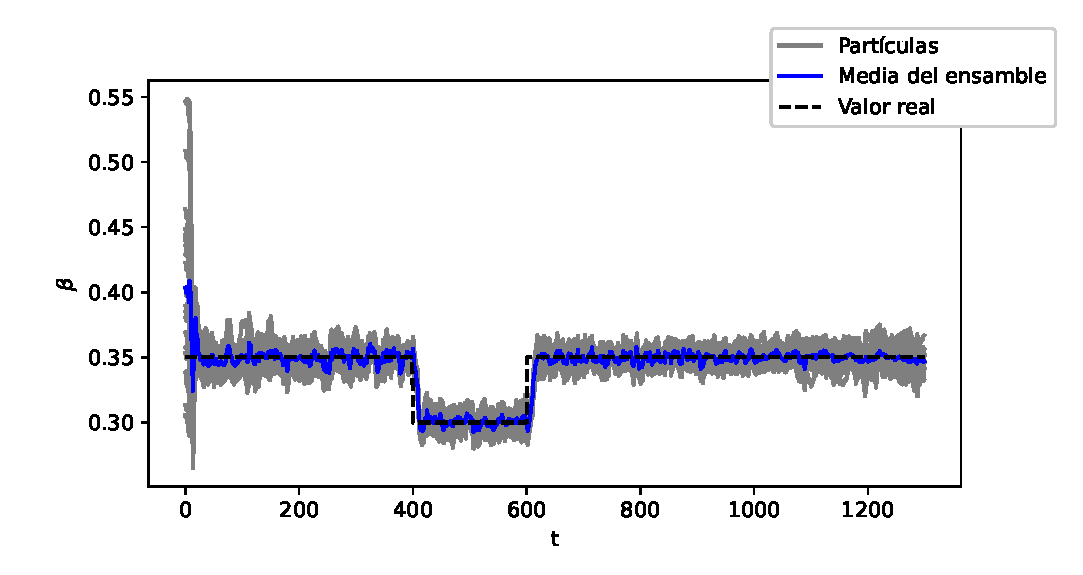
\includegraphics[width=0.75\textwidth]{figs/seird_online_em_aug_state_beta.eps}
    \caption{Valor real y estimaciones de la tasa de infección $\beta$}
    \label{fig:seird_online_em_aug_state_beta}
\end{figure}
\begin{figure}[h]
    \centering
    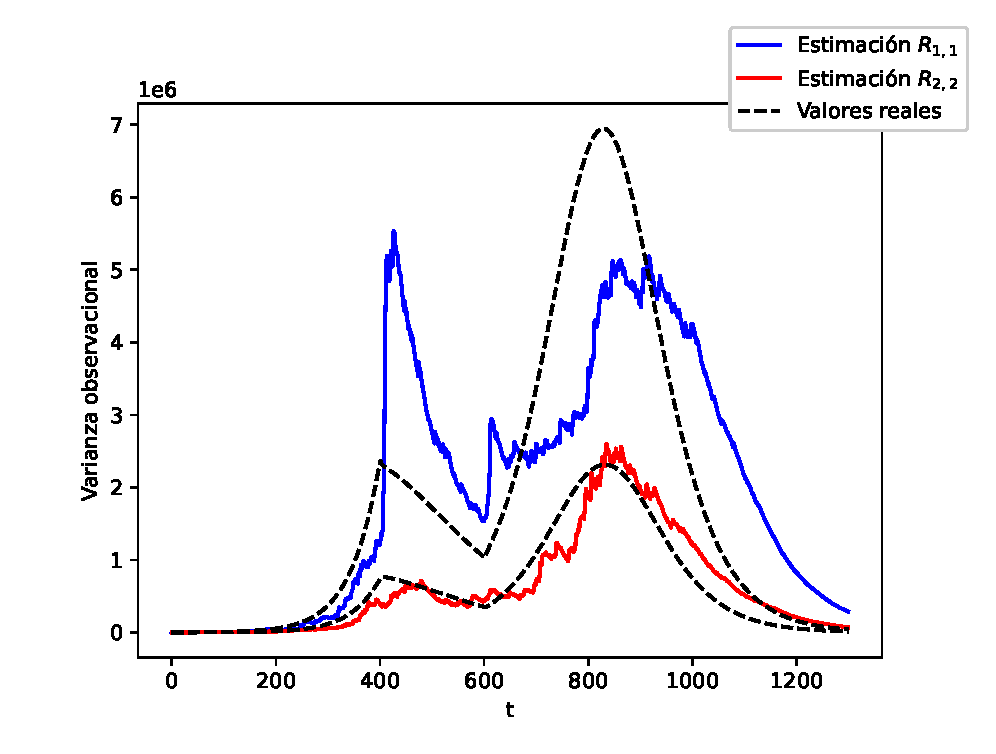
\includegraphics[width=0.75\textwidth]{figs/seird_online_em_aug_state_R.eps}
    \caption{Valores reales y estimados mediante EM online de las varianzas de errores observacionales. Estas corresponden a los dos valores de la diagonal de las matrices de covarianzas $\v R_t$}
    \label{fig:seird_online_em_aug_state_R}
\end{figure}

En la Figura \ref{fig:seird_online_em_aug_state_state_vars} se muestran los valores observados y reales de los infectados y muertos diarios junto con las correspondientes estimaciones. Se ve que el error observacional es proporcional al valor real como se especificó anteriormente y que las estimaciones de las variables sincronizan muy bien con los valores reales. El efecto de variación temporal sobre la tasa de infección $\beta$ explica el efecto de que el sistema produzca dos picos epidémicos. En la Figura \ref{fig:seird_online_em_aug_state_beta} se puede ver que las estimaciones de $\beta$ pueden capturar correctamente el cambio temporal del parámetro. Existe un retardo en las estimaciones para sincronizar luego de los cambios abruptos de la tasa de infección lo cual es habitual para técnicas de estado aumentado debido a que la asimilación tiene cierta inercia hacia valores previos y esto se corrige a medida que las observaciones se van asimilando. Finalmente, en la Figura \ref{fig:seird_online_em_aug_state_R} tenemos las estimaciones de $\v R_t$ producidas por el EM \textit{online} junto a los valores reales utilizados para generar las observaciones. A pesar de haber desvíos sustanciales de las estimaciones respecto a las trayectorias reales es evidente que el algoritmo EM percibe los cambios en $\v R_t$ y da aproximaciones que están en la misma escala. En este experimento utilizamos una tasa de aprendizaje $\alpha = 0.6$ lo que configura al algoritmo para tener ``poca memoria'' dándole más importancia a las observaciones que se están siendo procesadas y no tanto a las estimaciones anteriores. Realizamos réplicas de este mismo experimento con otros valores de $\alpha$ y se obtienen estimaciones menos ruidosas pero que reaccionan más lentamente a los cambios del parámetro.

Al error observacional lo consideraremos Gaussiano y aditivo mientras que a $\v R_t$, la matriz que especifica su varianza a tiempo $t$, la consideraremos diagonal, es decir sin correlación entre los errores. La varianza para el error en la primera variable observada la tomaremos proporcional a los infectados confirmados diarios,  i.e., $(\v R_t)_{1,1} \propto I_{tot}(t) - I_{tot}(t-1)$. Análogamente, para la segunda variable observada tomamos $(\v R_t)_{2,2} \propto D(t) - D(t-1)$. El parámetro $\beta$ será definido como una función constante a trozos. En particular, tendrá un valor de $0.35$ en toda la ventana temporal excepto por el intervalo donde $t \in (400, 600)$ donde su valor será $0.3$. Esto tiene el efecto de que el número de casos aumente, después amaine temporalmente para luego volver a crecer. Esta configuración para $\beta$ y $\v R_t$ se utilizará para generar las observaciones sintéticas pero será desconocida para el sistema de asimilación: $\beta$ se estimará mediante estado aumentado mientras que $\v R_t$ a través del EM \textit{online}.

\subsection{Experimento: datos COVID-19 de Argentina}
Como demostración de la potencial viabilidad de la técnica en modelos epidemiológicos realizamos otro experimento similar al de la Sección \ref{sec:online_em_seird_synthetic} pero utilizando los datos de COVID-19 en Argentina provistos por el Ministerio de Salud. El experimento tiene una configuración similar al de observaciones sintéticas que describimos anteriormente pero incorporamos además la tasa de mortalidad que llamaremos $\gamma_D$ y es computable como $(1-\alpha) \gamma_I I$ según las Ecuaciones \ref{eq:seird}.

Cuando se tienen parámetros en el estado aumentado (tal como se expone en la sección \ref{sec:augmented_state}) las caminatas aleatorias que se utilizan para que las estimaciones exploren el espacio paramétrico tienen el efecto de actuar como error de modelo. Por lo tanto, estas interactúan con el resto del sistema, con las estimaciones de $\v R$, y con el comportamiento de la media y dispersión de las variables de estado (ver Sección \ref{sec:model_obs_error}). En este experimento parametrizamos las caminatas aleatorias con un valor $\sigma^2$ de modo que la amplitud de los pasos es Gaussiana con media 0 y varianza $\sigma^2$ para $\beta$ y $\sigma^2/100$ para $\gamma_D$. Para estudiar su efecto corrimos el experimento para distintos valores de $\sigma^2$. 

En la Figura \ref{fig:seird_vars_arg_data} se grafican los infectados y muertos diarios observados y estimados para el caso de $\sigma^2 = 0.015$. Las trayectorias estimadas están prácticamente superpuestas a las observaciones y la escala impide apreciar la dispersión del ensamble sin embargo este no está colapsado. Los resultados para otros valores de $\sigma^2$ son similares pero la dispersión del ensamble tiende a ser menor cuando se aumenta su valor.

Las estimaciones de $\beta$ y $\gamma_D$ están en la Figura \ref{fig:seird_params_arg_data}. El comportamiento global de los parámetros es similar para todos los valores de $\sigma^2$ pero a medida que este valor aumenta las estimaciones son más ruidosas y con mayor varianza.
La tasa de infección es mayor al comienzo de la pandemia y alrededor de los picos de casos, notablemente en el que corresponde a finales de 2021. Por otro lado la tasa de mortalidad es mayor al comienzo de la ventana temporal y se va reduciendo en el tiempo de manera que el incremento en muertos en la última ola se explicaría según este modelo por el aumento de casos pero no por una mayor letalidad de la enfermedad.

Finalmente, en la Figura \ref{fig:seird_R_arg_data} se pueden ver las estimaciones de las varianzas de los errores observacionales $(\v R_t)_{1,1}$ y $(\v R_t)_{2, 2}$. En este caso es notable como el valor de $\sigma^2$ afecta a las estimaciones que produce el EM \textit{online}: el comportamiento es muy similar para distintos valores de $\sigma^2$ pero la escala es muy diferente. Esto se debe a la interacción entre el error de modelo y observacional. Es esperable que mientras mayor sea el error de modelo el sistema le de más importancia a las observaciones. El error que corresponde a la primera variable observada, los infectados acumulados, tiene un pico notable alrededor de la primera ola y otro en la ola de finales de 2021 pero este último se hace menos importante a medida que aumenta $\sigma^2$. Por su parte, el error que corresponde a los fallecidos acumulados es mayor al comienzo de la pandemia y luego se reduce y se estabiliza.

Los resultados dependen de la elección de las caminatas aleatorias en los parámetros dentro del estado aumentado ya que estos tienen el efecto de inyectar error de modelo al sistema. De hecho, podemos ver que al aumentar el valor de $\sigma^2$ se pierde credibilidad en el modelo porque este pasa tener mayor error. Esto resulta en que el sistema de asimilación de datos de mayor importancia a las observaciones y que se reduzca el error observacional estimado por el EM \textit{online}. En la figura \ref{fig:seird_params_arg_data} se aprecia que al aumentar la varianza de las caminatas aleatorias las estimaciones de los parámetros se hacen más ruidosas: esto es un comportamiento típico de sobreajuste las observaciones. El sistema le da demasiada credibilidad a los datos y por lo tanto las trayectorias de las variables de estado (incluidas las del estado aumentado) absorben el error de las observaciones.

\begin{figure}[h]
    \centering
    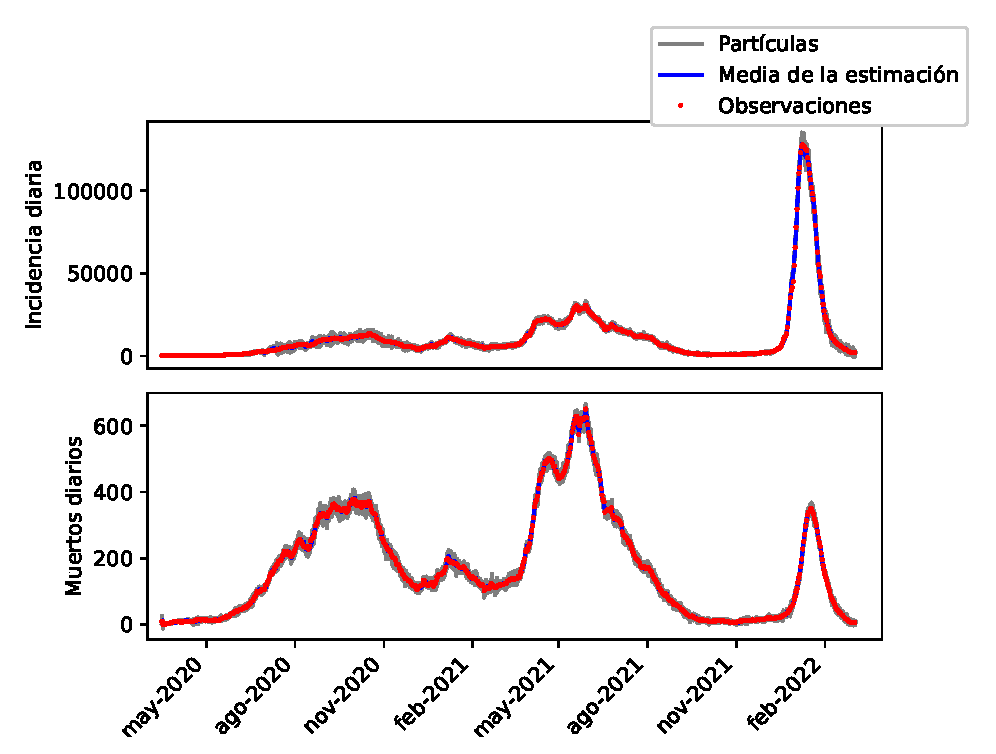
\includegraphics[width=0.75\textwidth]{figs/seird_online_em_aug_state_state_vars_arg_data.eps}
    \caption{Observaciones y estimaciones para los infectados diarios (incidencia diaria) y muertos diarios utilizando el modelo SEIRD sobre los datos de COVID-19 en Argentina}
    \label{fig:seird_vars_arg_data}
\end{figure}
\begin{figure}[h]
    \centering
    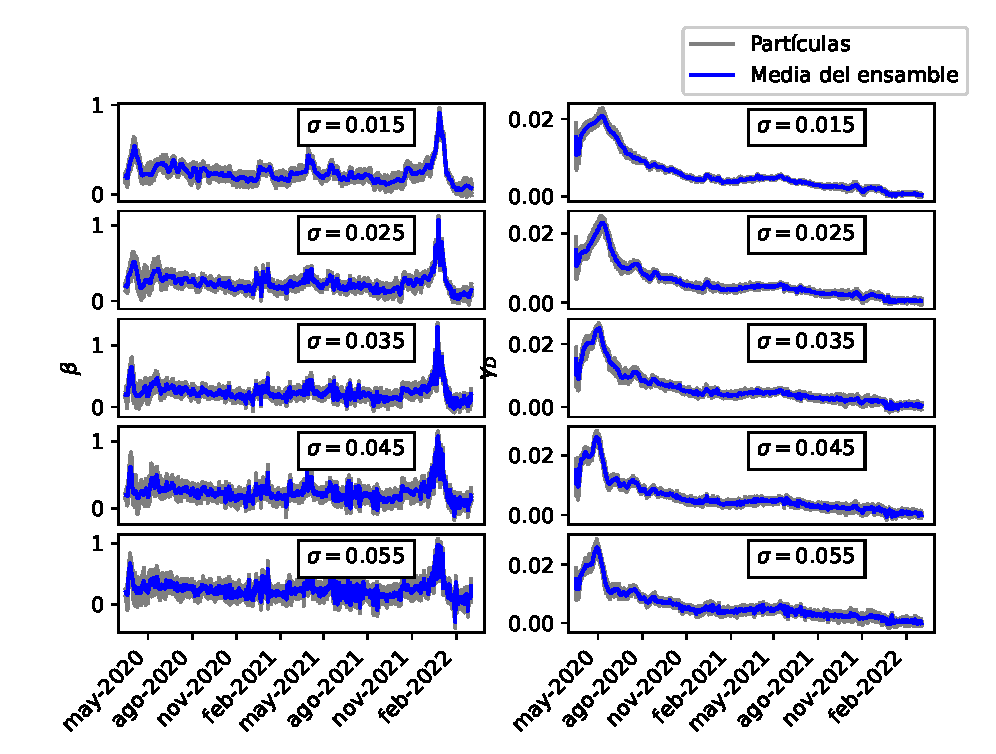
\includegraphics[width=0.75\textwidth]{figs/seird_online_em_aug_state_params_arg_data_sigmas.eps}
    \caption{Estimaciones de la tasa de infección $\beta$ y la tasa de fatalidad $\gamma_D$}
    \label{fig:seird_params_arg_data}
\end{figure}
\begin{figure}[h]
    \centering
    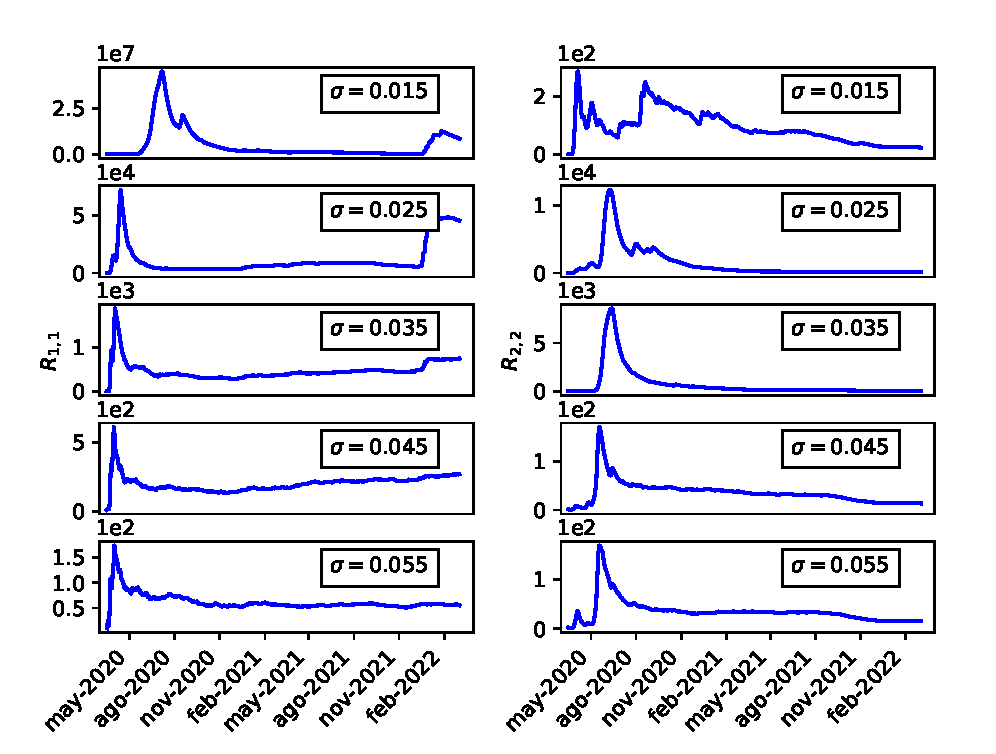
\includegraphics[width=0.75\textwidth]{figs/seird_online_em_aug_state_R_arg_data_sigmas.eps}
    \caption{Estimaciones del EM online de las varianzas de errores observacionales. Estas corresponden a los dos valores de la diagonal de las matrices de covarianzas $\v R_t$}
    \label{fig:seird_R_arg_data}
\end{figure}

\subsection{Discusión}

Diseñamos estos experimentos para mostrar la potencial viabilidad del EM \textit{online} para estimación de errores en sistemas de asimilación de datos sobre modelos epidemiológicos. Este aspecto es habitualmente pasado por alto en trabajos de inferencia mediante en este tipo de sistema. En el experimento con observaciones sintéticas, salvo por la parametrización que se calibra con estado aumentado, el modelo utilizado es el mismo que se usa para generar los datos. En el caso de tener datos reales no es posible especificar un modelo perfecto por lo que los parámetros en el estado aumentado cumplen el rol de calibrar otras posibles deficiencias del modelo. Los resultados obtenidos evidencian la interdependencia entre el error observacional y de modelo y como estos afectan la performance general de las estimaciones que produce el sistema. Una posibilidad es incorporar error de modelo aditivo y estimar su matriz de covarianza $\v Q_t$ con el EM \textit{online} y de hecho algunos experimentos preliminares sugieren que esto es posible. Además las varianzas de las caminatas aleatorias en el estado aumentado podrían potencialmente ser estimadas de manera adaptativa como parte de la matriz $\v Q_t$. Otra posibilidad más sencilla para dar cuenta del error de modelo es la utilización de un factor de inflación en el ensamble (ver Sección \ref{sec:enkf}).
